\chapter{Introduction}
\label{sec:Introduction}

Traditionally, software is written for sequential computation. A problem is broken down into a series of instrcutions. Those instructions are executed sequentially on a single processor. In this scenario, only one instruction is executed at any given moment in time~\cite{barney2010introduction}.\\
Parallel computing is a type of computation in which calculations are carried out simultaneously to solve a computational problem~\cite{Almasi:1989:HPC:160438}. In parallel computing, a problem is broken down into discrete parts that can be solved concurrently. Each part includes a series of instructions. Instructions for each part of the problem are executed in parallel on different processors. This this scenario, a control mechanism among all the processors is needed.


\section{Parallel Architectures}
Parallel computers can be classified in different ways. Flynn's taxonomy is one of the more widely used classification of different computer architectures proposed by Michael J. Flynn in 1966\cite{5009071,44900}. This classification is based on the number of concurrent instruction streams and data streams available in the architecture.
There are four categories defined:

\begin{enumerate}
  \item \textbf{Single Instruction, Single Data Stream (SISD)}\\
    In this architecture, a single processor executes a single instruction stream and only one data stream is available as an input during any given clock cycle. This is basically a serial computer.
  \item \textbf{Single Instruction, Multiple Data Streams (SIMD)}\\
    This architecture describes computers with multiple processing elements which execute the same instruction at any given clock cycle. Each processing unit can use a different data stream.
  \item \textbf{Multiple Instruction, Single Data Stream (MISD)}\\
    In this architecture, multiple processing units operate on a single data stream, each one having a separate set of instructions. This architecture is almost non-existent.
  \item \textbf{Multiple Instruction, Multiple Data Streams (MIMD)}\\
    In this architecture, multiple independent processors execute different instructions on different data streams at the same time. Execution can be synchronous or asynchronous. This is the most generic category. Most current supercomputers fall under this category.
\end{enumerate}

\section{Parallel Computer Memory Architectures}
Main memory in a parallel computer is either shared or distributed~\cite{patterson2013computer}.

\subsection{Shared Memory}
In a shared memory parallel computer, the memory is shared between all processing elements as a single global address space. Multiple processors can share the same memory resources and operate independently. Changes in a memory location by one processor are visible to all other processors.\\ 
Furthermore, shared-memory architectures can be classified as symmetric multiprocessors with uniform memory access (UMA) or as non-uniform memory access (NUMA) architectures based on memory access time~\cite{kshemkalyani2008distributed,sutter2005free}.

\begin{itemize}
\item \textbf{Uniform Memory Access (UMA)}\\
  This category is most known by Symmetric Multiprocessor (SMP) machines. SMPs have identical processors with equal access time to memory. Figure \ref{fig:shared_memory_UMA} demonstrates a typical UMA architecture.\\
  \begin{figure}[h!]
    \centering
    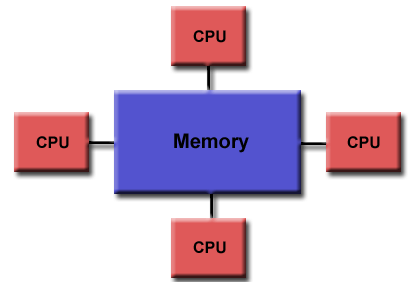
\includegraphics[scale=0.6]{images/shared_mem.png}
    \caption{Shared Memory (UMA)}
    \label{fig:shared_memory_UMA}
  \end{figure}

\item \textbf{Non-Uniform Memory Access (NUMA)}\\
  Typically, these are made by physically connecting two or more SMPs. This way, one SMP can access memory of another SMP directly. However, access time to all memories is not equal to all processors.
  
  \begin{figure}[h!]
    \centering
    
\includegraphics[scale=0.6]{images/numa.png}
    \caption{Shared Memory (NUMA)}
    \label{fig:shared_memory_NUMA}
  \end{figure}

\end{itemize}


\subsection{Distributed Memory}
Each processing element has its own local memory. Therefore, there is no global address space. To connect inter-process memory units, a communication network is needed.
Each processor operates independently. Changes that a processor makes to its local memory have no effect on the memory of other processors. If a processor needs to access data in another processor's memory, the programmer needs to explicitly define the communication mechanism.

\begin{figure}[h!]
  \centering
  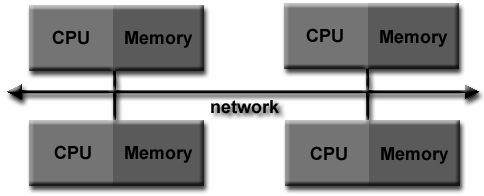
\includegraphics[scale=0.6]{images/distributed_mem.png}
  \caption{Distributed Memory}
  \label{fig:distributed_mem}
\end{figure}


\subsection{Hybrid Distributed-Shared Memory}

\begin{figure}[h!]
  \centering
  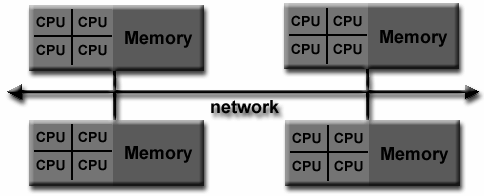
\includegraphics[scale=0.6]{images/hybrid_mem.png}
  \caption{Hybrid Distributed-Shared Memory}
  \label{fig:hybridd_mem}
\end{figure}



\section{Parallel Programming Models}
The programming model is an abstraction that defines the hardware and the form of programming language or API used for writing parallel programs.
Parallel programming models can be divided into two broad areas: Process interaction and problem decomposition.~\cite{parallelprogrammingmodels}
\begin{itemize}
\item \textbf{Process Interaction}\\
  Parallel processes need to communicate with each other. The mechanism that they use for the communication is described as process interation. Two main types of process interaction are shared memory and message passing. The interaction could also be implicit.
  \begin{itemize}
  \item \textbf{Shared Memory}\\
    In this model, parallel processes share a global address space which they all read and write to. Since these operations are asynchronous, protection mechanisms like locks and semaphores are needed to control concurrent access.
  \item \textbf{Message Passing}\\
    In this model, parallel tasks exchange data through sending and receiving messages to and from one another. These communications can be synchronpus or asynchronus.
  \item \textbf{Implicit}\\
    In this model, process interactions are not visible to the programmer. Usually, the compiler or the runtime is responsible for performing the interations.
  \end{itemize}
\item \textbf{Problem Decomposition}\\
Problem decomposition describes the way processes are expressed to break down a large problem~\cite{Quinn:2003:PPC:1211440}.
  \begin{itemize}
  \item \textbf{Task Parallelism}\\
    The main focus of a task based parallelism is on processes or threads as individual units of execution. This is a natural way to express message passing communication.
  \item \textbf{Data Parallelism}\\
    In task-parallel models the data is usually structured in an array. A set of tasks will operate independently on separate partitions of the data.     
  \end{itemize}
\end{itemize}


\section{Message Passing Interface (MPI)}
Message Passing Interface (MPI) is a language-independent communication protocol used for programming in parallel environments. ``MPI is a specification for a standard library for message passing that was defined by the MPI Forum, a broadly based group of parallel computer vendors, library writers, and applications specialists.''~\cite{gropp1996high} MPI has become a de facto standard for communication aming processes running on a distributed memory system.

``The goal of the Message Passing Interface is to establish a portable, efficient, and flexible standard for message passing that will be widely used for writing message passing programs. As such, MPI is the first standardized, vendor independent, message passing library. The advantages of developing message passing software using MPI closely match the design goals of portability, efficiency, and flexibility. MPI is not an IEEE or ISO standard, but has in fact, become the ``industry standard'' for writing message passing programs on HPC platforms.''~\cite{barker2015message} There are several implementations of MPI, including some that are in the public domain and some proprietary implementations from companies like HP, Intel, and Microsoft.


\section{Runtime Environments and MPI Jobs}
High performance computing systems are growing toward hundreds of thousands to million node machines, utilizing the computing power of billions of cores. Running parallel applications on such large machines efficiently will require optimized runtime environments that are scalable and resilient. Considering a future where MPI remains a major programming paradigm, the MPI implementations will have to seamlessly adapt to launching and managing large scale applications on resources considerably larger than today.~\cite{bosilca2011scalability}

\section{Challenges for Runtime Environments}
Multi and many core chip architectures in large scale supercomputers pose several new challenges to designers of operating systems and runtime environments.\\
``Operating systems and runtime environments on supercomputers have similar goals: both seek to provide an environment for executing applications in a scalable and high-performing way. Achieving this goal often requires minimizing the layers of indirection between the application and the architecture.''~\cite{Hoefler:2012:OSR:2237840.2237848}\\
Developing a software environment to support high performance computing applications in today's distributed systems poses a significant challenge. The runtime environment (RTE) must be capable of supporting heterogeneous operations, scale from one to large numbers of processors in an efficient manner, and provide strategies for dealing with fault scenarios that are expected of computing systems effectively. Furthermore, the runtime must be easy to use, providing users with a transparent interface to the computing environment in a manner that avoids the need to customize applications when moving between specific computing resources.~\cite{Castain2008153}

\section{Organization of the Document}
Chapter 2 provides a background and the state of art approaches to parallel runtime enviroment challenges. Open MPI as an implementation of choice will be introduced. We will discuss the project features and its architecture. Open Runtime Environment (ORTE), the current runtime environment for Open MPI project, and its features will be discussed in detail in secion 2.2. ParalleX and High Perfomance ParalleX (HPX) will be presented in section 2.3. Chapter 3 covers the design philosophy, architecture, and implementation of our runtime environment for Open MPI (HPX-RTE) in sections 3.1, 3.2, and 3.3 accordingly.

